\documentclass{beamer}
\usepackage{pgfpages}
\usepackage[backend=bibtex]{biblatex}
\usepackage{multicol}
\usepackage{multimedia}
\usepackage[absolute,overlay]{textpos}
\usepackage{parskip}
\usepackage{hyperref}
\usepackage{lmodern}
\usepackage{bbding}
\usepackage[absolute,overlay]{textpos}
\usepackage{framed} %Used to shade important equations, color devined with shadecolor
\hypersetup{colorlinks=true, urlcolor=blue}
\setlength{\parskip}{\smallskipamount}
\colorlet{shadecolor}{cyan}
%\usepackage[texcoord,grid,gridunit=mm,gridcolor=red!10,subgridcolor=green!10]{eso-pic} %DELETE when done with grid
\setbeameroption{hide notes} % Only slides
%\setbeameroption{show only notes} % Only notes
%\setbeameroption{show notes on second screen=right} % Both
%\bibliography{../../papers/references.bib}
\setbeamerfont{footnote}{size=\tiny}
%\AtEveryCitekey{\clearfield{title}}

%
% Choose how your presentation looks.
%
% For more themes, color themes and font themes, see:
% http://deic.uab.es/~iblanes/beamer_gallery/index_by_theme.html
%
\mode<presentation>
{
\usetheme{Warsaw}      % or try Darmstadt, Madrid, Warsaw, ...
\usecolortheme{default} % or try albatross, beaver, crane, ...
\usefonttheme{default}  % or try serif, structurebold, ...
\setbeamertemplate{navigation symbols}{}
\setbeamertemplate{caption}[numbered]
} 

\usepackage[english]{babel}
%\usepackage[utf8x]{inputenc} %Doesn't play well with biblatex
\usepackage{amssymb}
\usepackage{bm}
\usepackage{color}
\usepackage{graphicx}
\setbeamercovered{invisible}
\setbeamercovered{%
again covered={\opaqueness<1->{100}}} %This changes the opaqueness of each bullet

\newcommand{\red}[1]{{\color{red}{#1}}}
\newcommand{\checkH}[2]{\begin{textblock*}{1cm}(#1,#2){\Huge \red{\Checkmark}}\end{textblock*}}
\newcommand{\checkh}[2]{\begin{textblock*}{1cm}(#1,#2){\huge \red{\Checkmark}}\end{textblock*}}
\newcommand{\checkL}[2]{\begin{textblock*}{1cm}(#1,#2){\Large \red{\Checkmark}}\end{textblock*}}
\newcommand{\checkl}[2]{\begin{textblock*}{1cm}(#1,#2){\large \red{\Checkmark}}\end{textblock*}}
\renewcommand{\rm}[1]{\mathrm{#1}}

\title[{\color{white}{Chapters 5.1-3}}]{Physics 121: \\ Force}
\author{Cody Petrie}
\institute{Mesa Community College}
\date{}

\begin{document}

%\setbeamertemplate{frametitle}[default][center]
\begin{frame}
\titlepage
\end{frame}

% Uncomment these lines for an automatically generated outline.
%\begin{frame}{Outline}
%  \tableofcontents
%\end{frame}

% Commands to include a figure:
%\begin{figure}
%\includegraphics[width=\textwidth]{your-figure's-file-name}
%\caption{\label{fig:your-figure}Caption goes here.}
%\end{figure}

\begin{frame}{Reminder}
\begin{itemize}
   \item Go over the test
   \item Next HW is due next Thursday (28th of September). Covers chapter 5 on Forces.
\end{itemize}
\end{frame}

\begin{frame}{Chapter Preview}
\begin{center}
   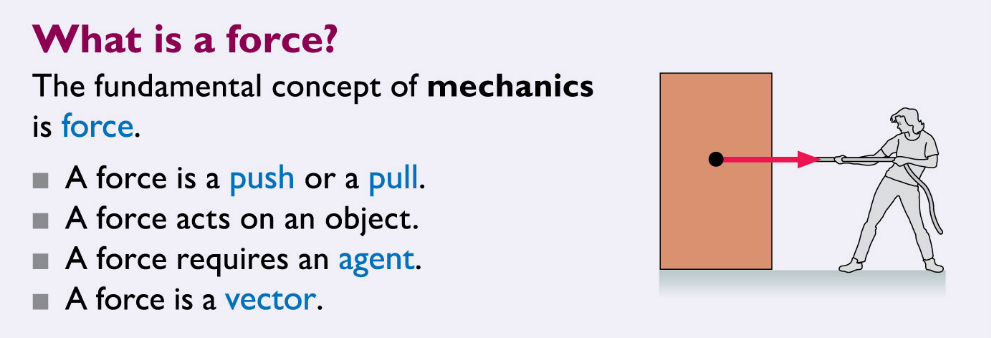
\includegraphics[width=\textwidth]{../figures/05_preview_01.png}
\end{center}
\end{frame}

\begin{frame}{Chapter Preview}
\begin{center}
   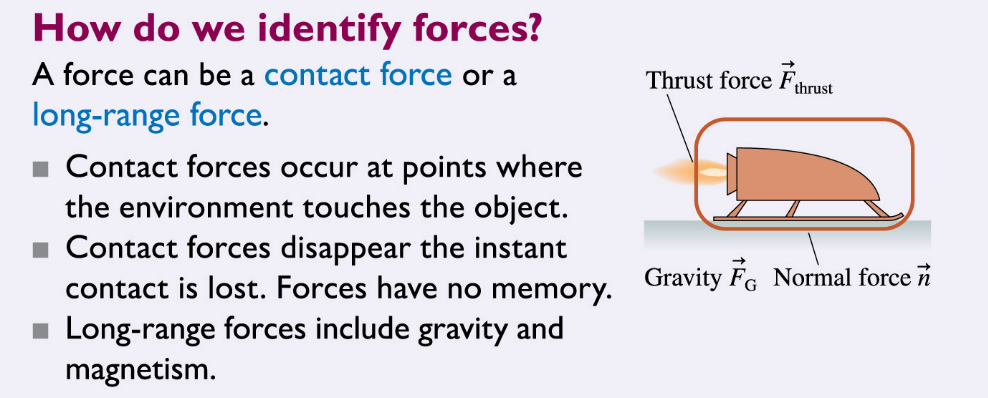
\includegraphics[width=\textwidth]{../figures/05_preview_02.png}
\end{center}
\end{frame}

\begin{frame}{Chapter Preview}
\begin{center}
   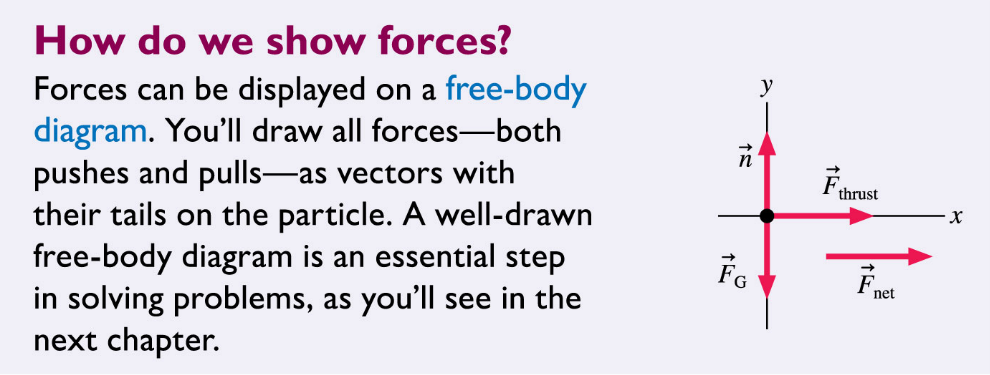
\includegraphics[width=\textwidth]{../figures/05_preview_03.png}
\end{center}
\end{frame}

\begin{frame}{Force}
\begin{columns}
\begin{column}{0.6\textwidth}
\begin{itemize}
   \item A force is a {\it push} or {\it pull}.
   \\~\\~\\~\\~\\
   \item A force acts on an {\bf object}, the thing that pushed and pulls act on.
   \item The object has a force {\it exerted} on it. The boxer exerted a force on the punching bag.
\end{itemize}
\end{column}
\begin{column}{0.4\textwidth}
\begin{center}
   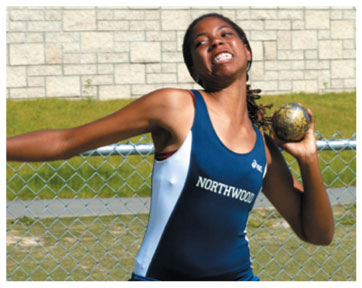
\includegraphics[width=0.95\textwidth]{../figures/05_Pg111_UnFigure1.jpg}
   \\~\\
   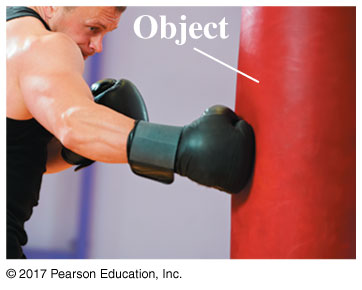
\includegraphics[width=0.95\textwidth]{../figures/05_Pg111_UnFigure2.jpg}
\end{center}
\end{column}
\end{columns}
\end{frame}

\begin{frame}{Force}
\begin{columns}
\begin{column}{0.4\textwidth}
\begin{center}
   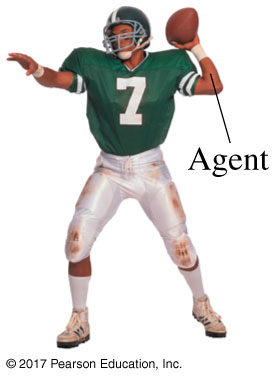
\includegraphics[width=0.85\textwidth]{../figures/05_Pg111_UnFigure3.jpg}
   \\~\\
   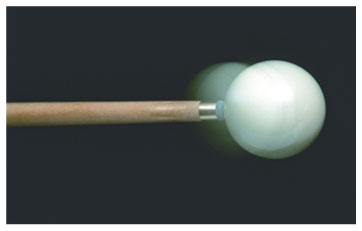
\includegraphics[width=0.95\textwidth]{../figures/05_Pg111_UnFigure4.jpg}
\end{center}
\end{column}
\begin{column}{0.6\textwidth}
\begin{itemize}
   \item A force is exerted on something by an {\bf agent}.
   \item If you throw or kick an object your hand or foot is the agent exerting the force on the object.
   \\~\\~\\~\\~\\~\\
   \item A force is a vector (all vector rules we have learned apply).
   \item To quantify the force (push or pull) you need both magnitude and direction.
\end{itemize}
\end{column}
\end{columns}
\end{frame}

\begin{frame}{Force}
\begin{columns}
\begin{column}{0.6\textwidth}
\begin{itemize}
   \item Forces come in two types. The first type is a {\bf contact force}.
   \item Contact forces need to touch a object to exert a force on it.
   \\~\\~\\~\\~\\~\\
   \item The second type is a {\bf long-range force} in which the agent doesn't tough the object. \red{Examples?}
   \item<2> Gravity or magnetism are examples of long-range forces.
\end{itemize}
\end{column}
\begin{column}{0.4\textwidth}
\begin{center}
   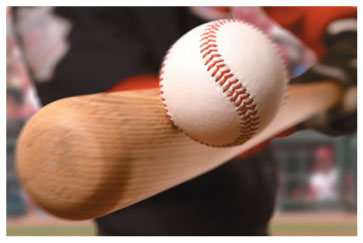
\includegraphics[width=0.85\textwidth]{../figures/05_Pg111_UnFigure5.jpg}
   \\~\\
   \uncover<2>{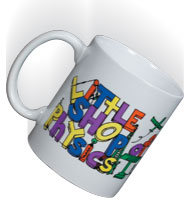
\includegraphics[width=0.95\textwidth]{../figures/05_Pg111_UnFigure6.jpg}}
\end{center}
\end{column}
\end{columns}
\end{frame}

\begin{frame}{Force}
\begin{itemize}
   \item How do you think we represent forces visually?
   \\~\\
\end{itemize}
\begin{center}
   \uncover<2>{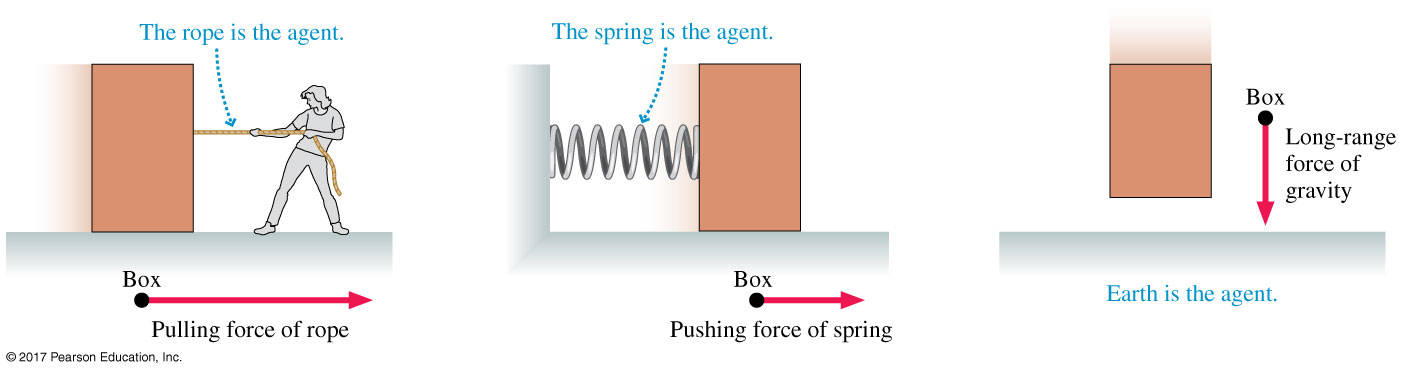
\includegraphics[width=\textwidth]{../figures/05_01_Figure.jpg}}
\end{center}
\end{frame}

\begin{frame}{Force}
\begin{itemize}
   \item Why am I not being ``forced" down by gravities force right now?
   \item<2> There is a force on me from the ground. These two forces must cancel out. Thus you must be able to add forces to come up with a {\it resulting force}.
   \item<3> The resulting force is called the {\bf net force}.
   \begin{equation*}
      \vec{F}_{net} \equiv \sum\limits_{i=1}^N \vec{F}_i = \vec{F}_1 + \vec{F}_2 + \ldots + \vec{F}_N
   \end{equation*}
   NOTICE THAT THIS IS VECTOR ADDITION.
\end{itemize}
\end{frame}

\begin{frame}{Quick Check}
\begin{center}
   There are two forces pulling on this box. Draw the force vectors on the box to find the net force on the box. Assume the forces are the same magnitude.\\
   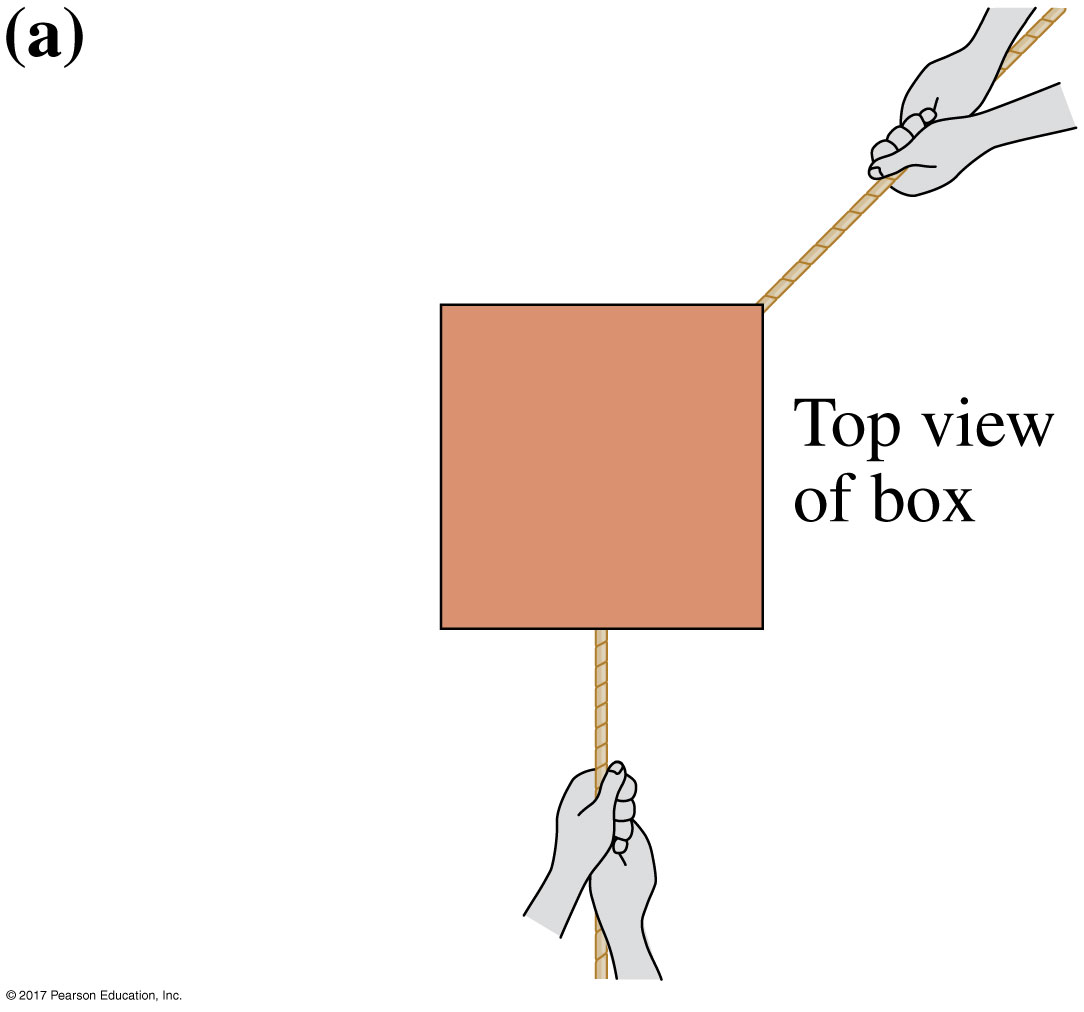
\includegraphics[width=0.47\textwidth]{../figures/05_02_FigureA.jpg}
   ~~
   \uncover<2>{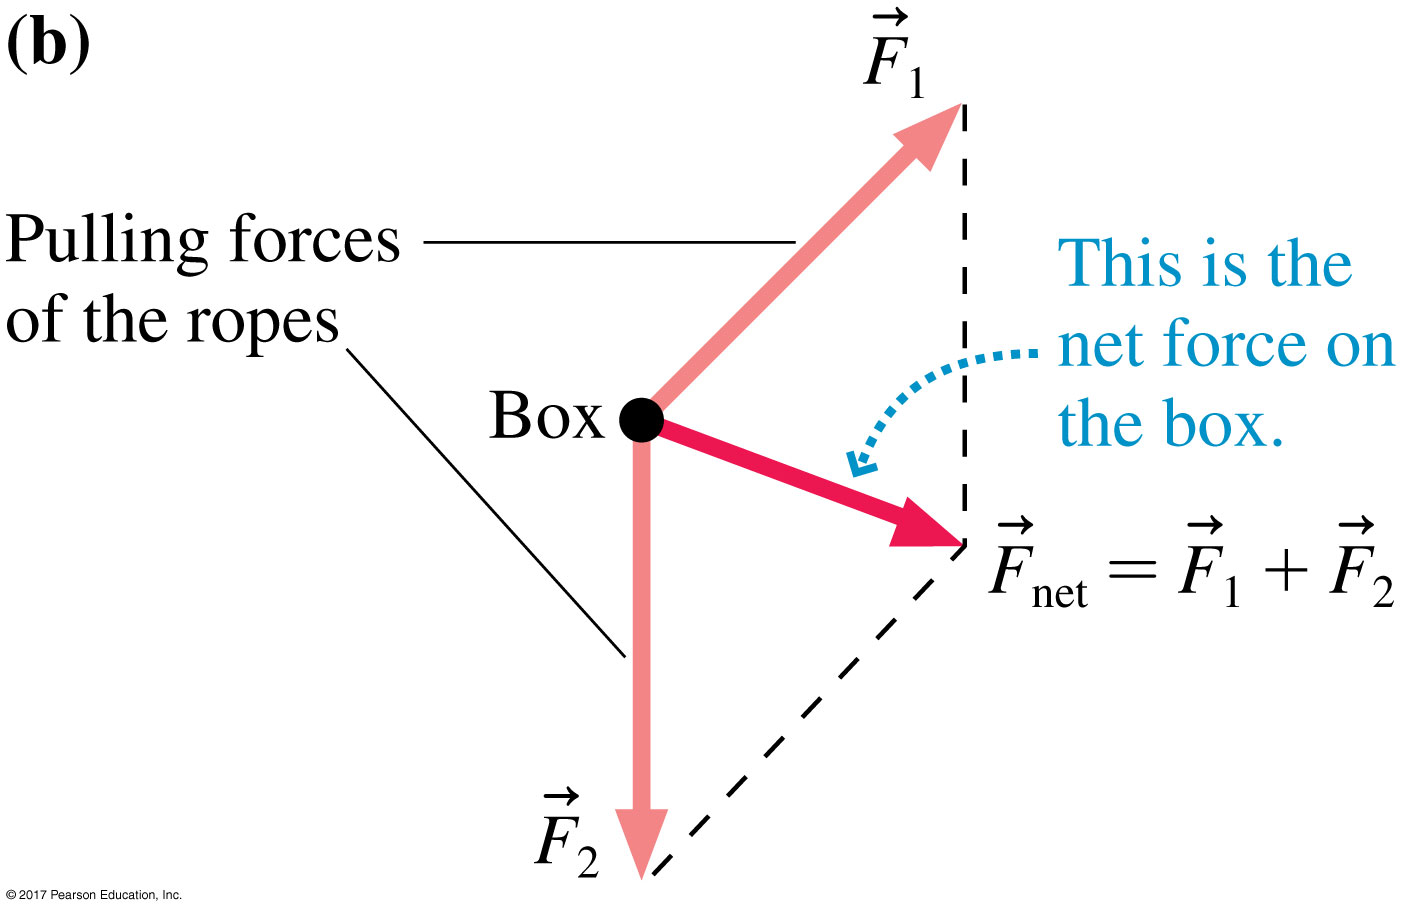
\includegraphics[width=0.48\textwidth]{../figures/05_02_FigureB.jpg}}
\end{center}
\end{frame}

\begin{frame}{Force}
\begin{center}
   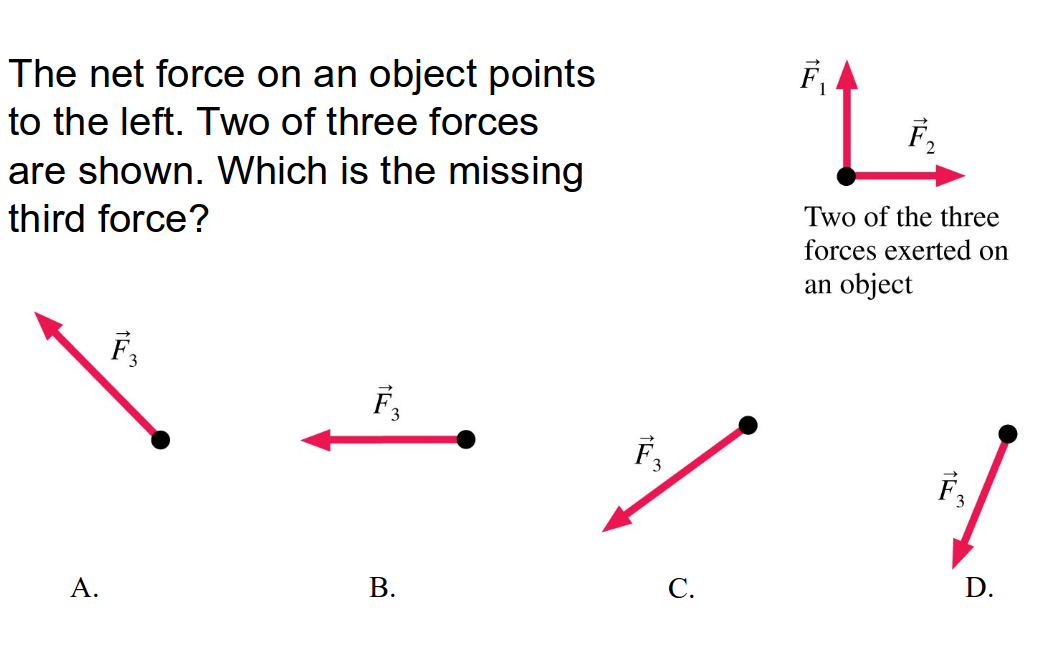
\includegraphics[width=\textwidth]{../figures/QC5_2.png}
   \only<2>{\checkL{7.6cm}{7.4cm}}
\end{center}
\end{frame}

\begin{frame}{Types of Forces - Gravity}
\begin{columns}
\begin{column}{0.5\textwidth}
\begin{itemize}
   \item The pull of a planet on an object near the surface is called the {\bf gravitational force}.
   \item The agent for the gravitational force is the entire planet.
   \item Gravity acts on all objects, whether moving or at rest.
   \item The gravitational force vector always points vertically downward.
\end{itemize}
\end{column}
\begin{column}{0.5\textwidth}
\begin{center}
   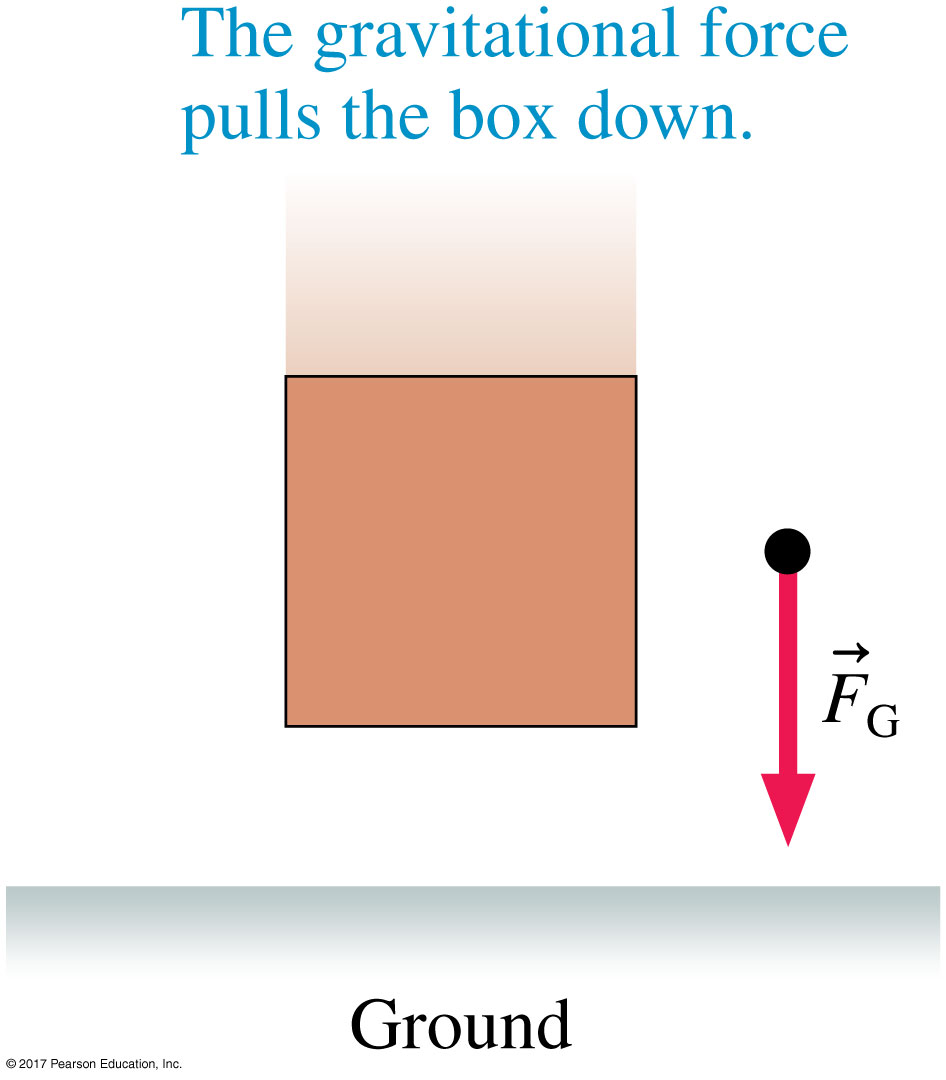
\includegraphics[width=\textwidth]{../figures/05_03_Figure.jpg}
\end{center}
\end{column}
\end{columns}
\end{frame}

\begin{frame}{Types of Forces - Spring Force}
\begin{columns}
\begin{column}{0.5\textwidth}
\begin{center}
   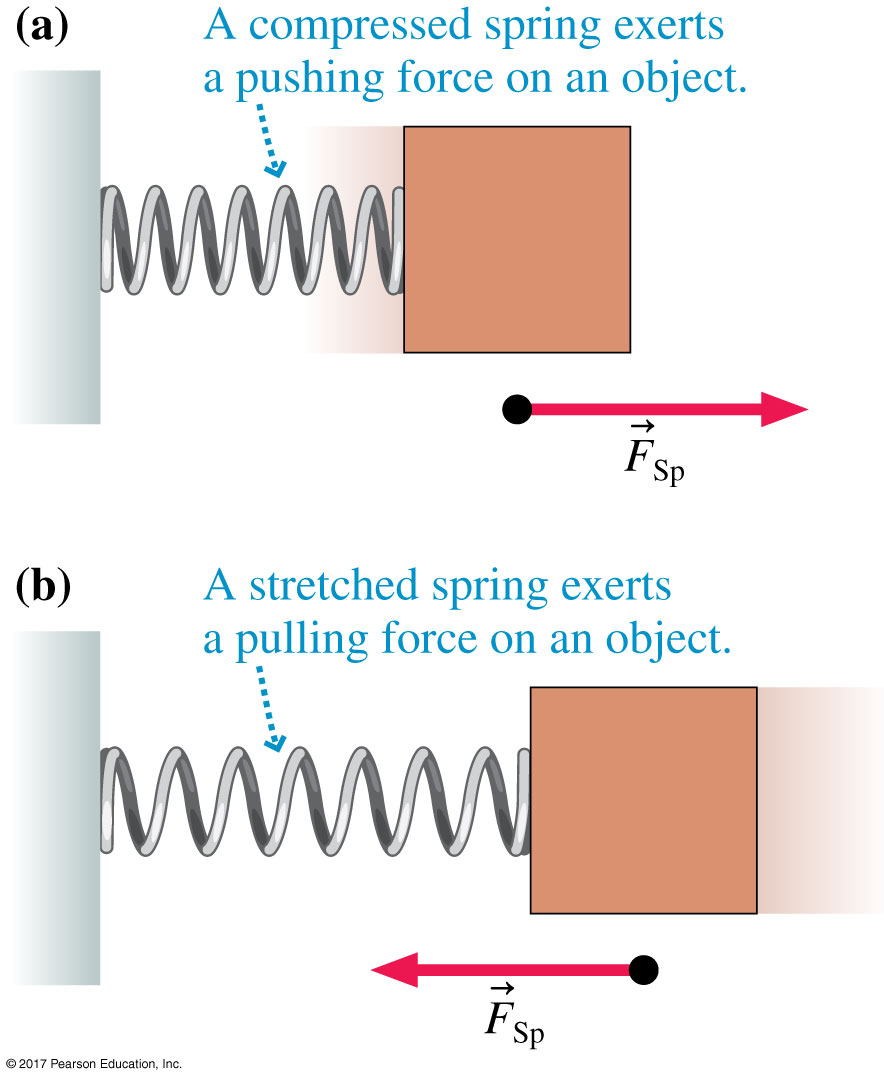
\includegraphics[width=\textwidth]{../figures/05_04_Figure.jpg}
\end{center}
\end{column}
\begin{column}{0.5\textwidth}
\begin{itemize}
   \item A spring can either push (when compressed) or pull (when stretched).
   \item Not all springs are metal coils.
   \item Whenever an elastic object is flexed or deformed in some way, and then ``springs" back to its original shape when you let it go, this is a {\bf spring force}.
\end{itemize}
\end{column}
\end{columns}
\end{frame}

\begin{frame}{Types of Forces - Tension}
\begin{itemize}
   \item When a string or rope or wire pulls on an object, it exerts a contact force called the tension force.
   \item The tension force is in the direction of the string or rope.
\end{itemize}
\begin{center}
   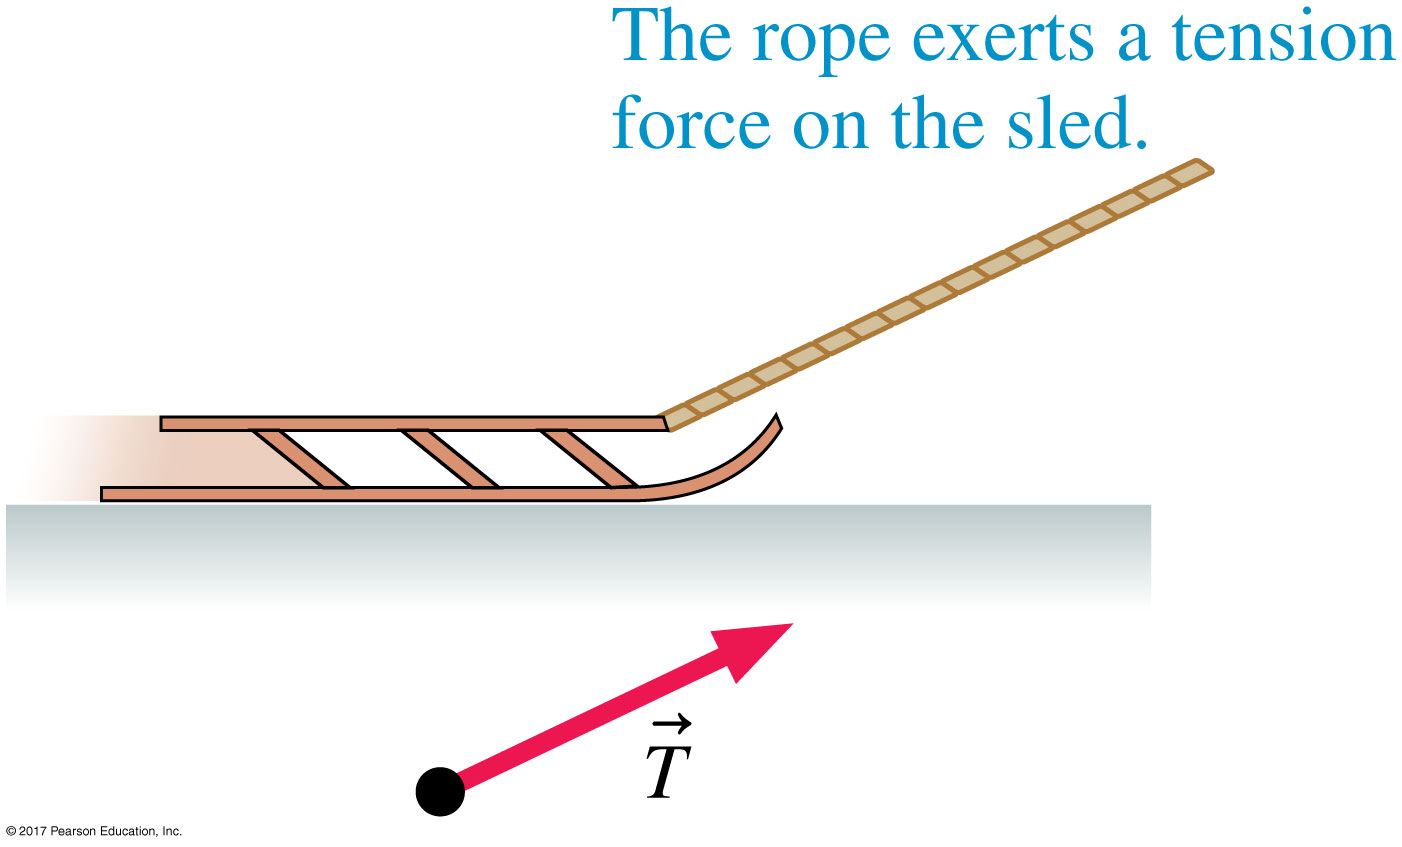
\includegraphics[width=\textwidth]{../figures/05_05_Figure.jpg}
\end{center}
\end{frame}

\begin{frame}{Types of Forces}
\begin{center}
   What exactly is happening when you pull on a rope attached to an object? How does the force you exert transfer through the rope?
   \uncover<2>{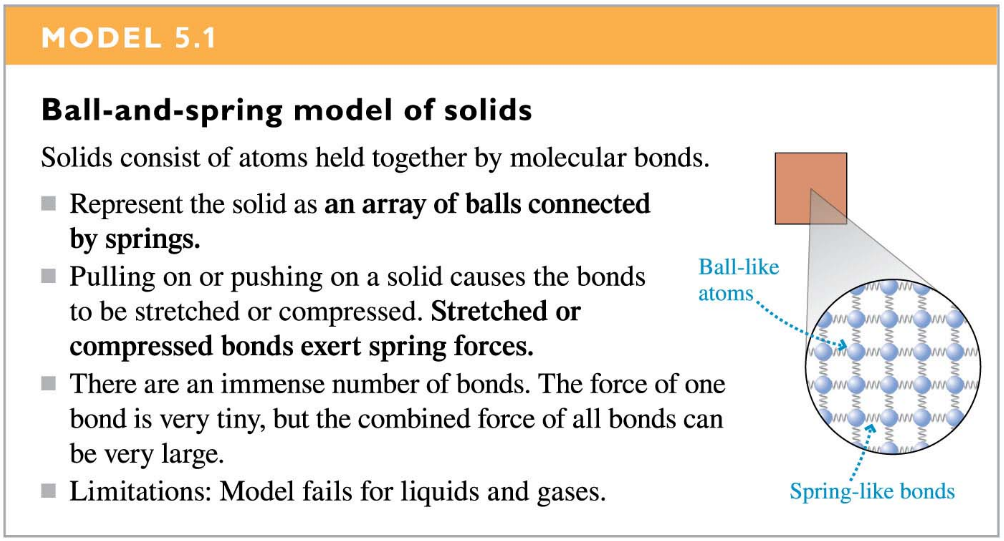
\includegraphics[width=\textwidth]{../figures/model5_1.png}}
\end{center}
\end{frame}

\begin{frame}{Quick Check}
\begin{center}
   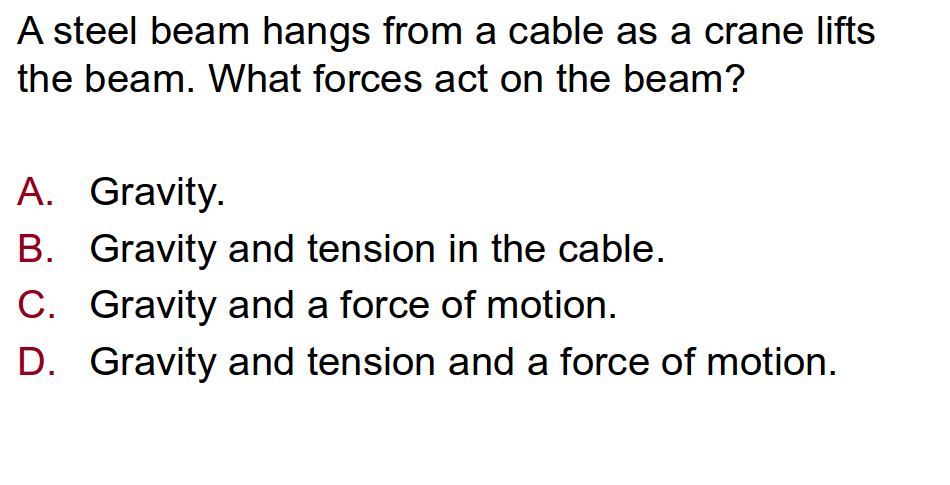
\includegraphics[width=\textwidth]{../figures/QC5_3.png}
\end{center}
\only<2>{\checkL{0.9cm}{4.4cm}}
\end{frame}

\begin{frame}{Types of Forces - Normal Force}
\begin{columns}
\begin{column}{0.6\textwidth}
\begin{itemize}
   \item When an object sits on a table, the table surface exerts an upward 
contact force on the object.
   \item This pushing force is directed {\it perpendicular} to the surface, and thus is called the {\bf normal force}.
   \item A table is made of atoms joined together by molecular bonds which can be modeled as springs.
   \item Normal force is a result of many molecular springs being compressed ever so slightly.
\end{itemize}
\end{column}
\begin{column}{0.4\textwidth}
\begin{center}
   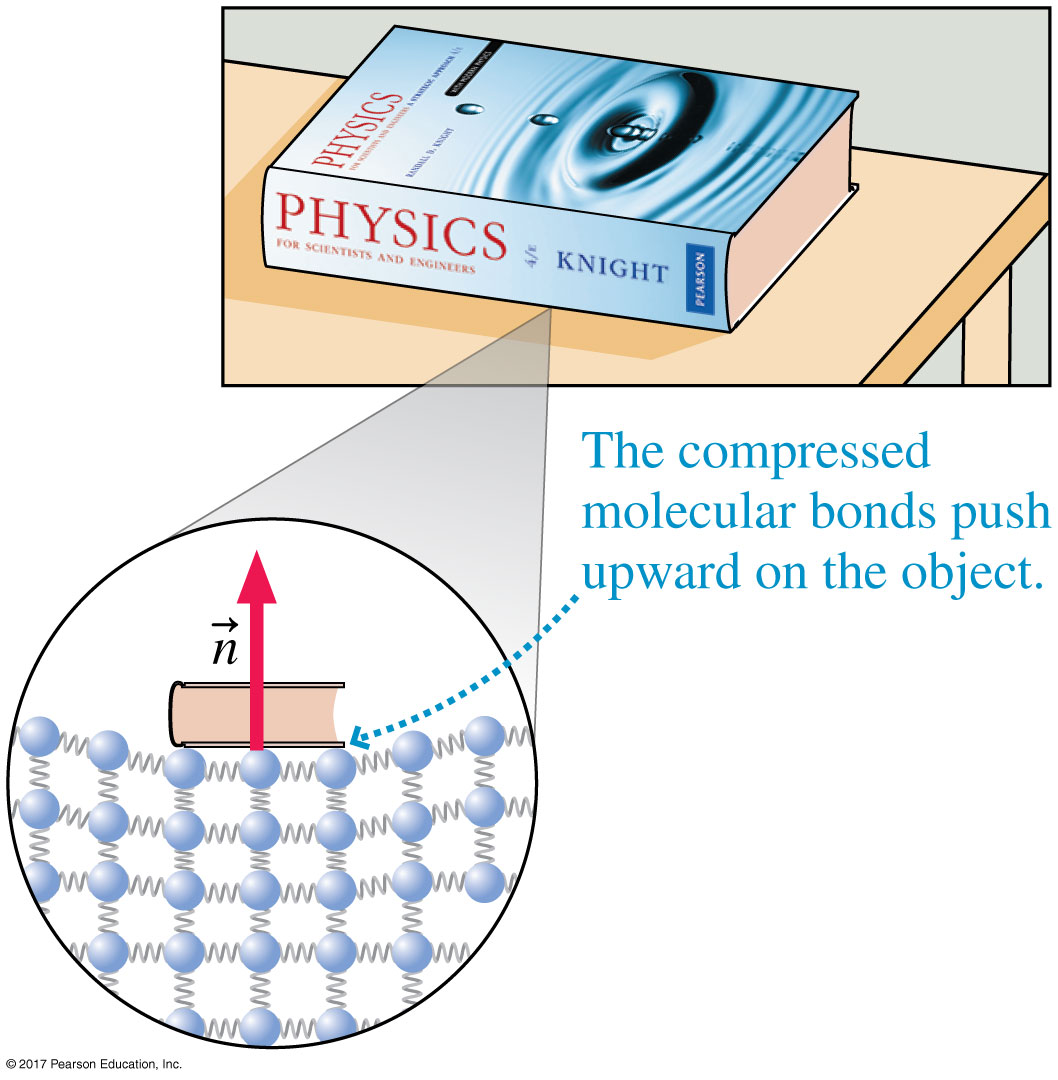
\includegraphics[width=\textwidth]{../figures/05_06_Figure.jpg}
\end{center}
\end{column}
\end{columns}
\end{frame}

\begin{frame}{Types of Forces - Normal Force}
\begin{itemize}
   \item The normal force is perpendicular to the surface regardless the angle it makes with the object.
   \item Suppose a frog sits on an inclined surface. The surface exerts a tilted normal force on the frog.
\end{itemize}
\begin{center}
   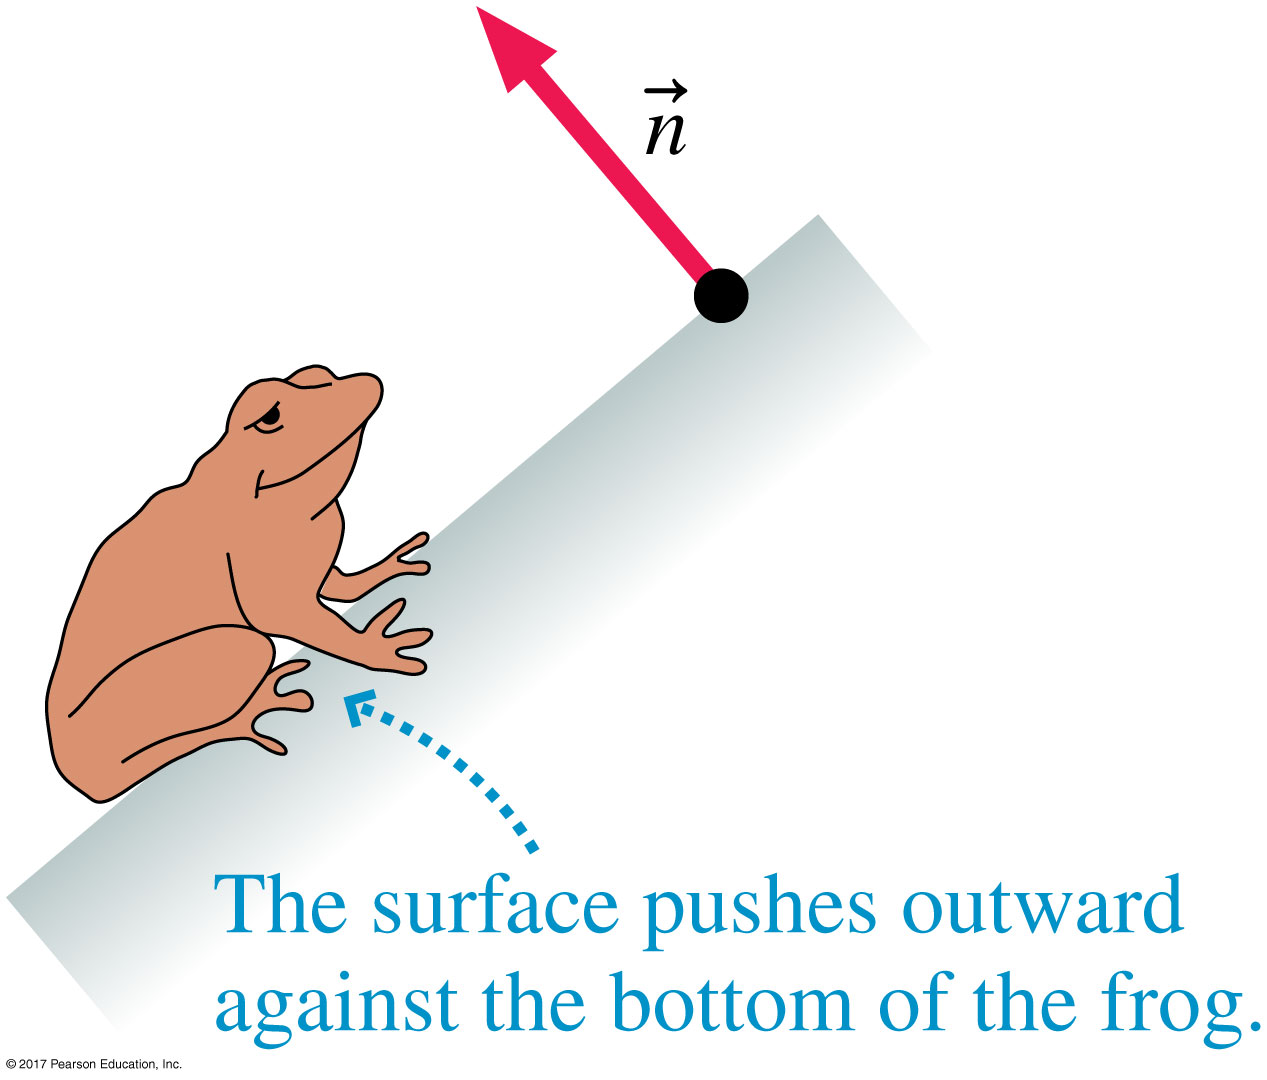
\includegraphics[width=0.6\textwidth]{../figures/05_07_Figure.jpg}
\end{center}
\end{frame}

\begin{frame}{Types of Forces - Kinetic Friction}
\begin{columns}
\begin{column}{0.6\textwidth}
\begin{itemize}
   \item When an object slides along a surface, the surface can exert a contact force which opposes the motion.
   \item This is called sliding friction or {\bf kinetic friction}.
   \item The kinetic friction force is directed {\it tangent to the surface}, and {\it opposite to the velocity} of the object relative to the surface.
\end{itemize}
\end{column}
\begin{column}{0.4\textwidth}
\begin{center}
   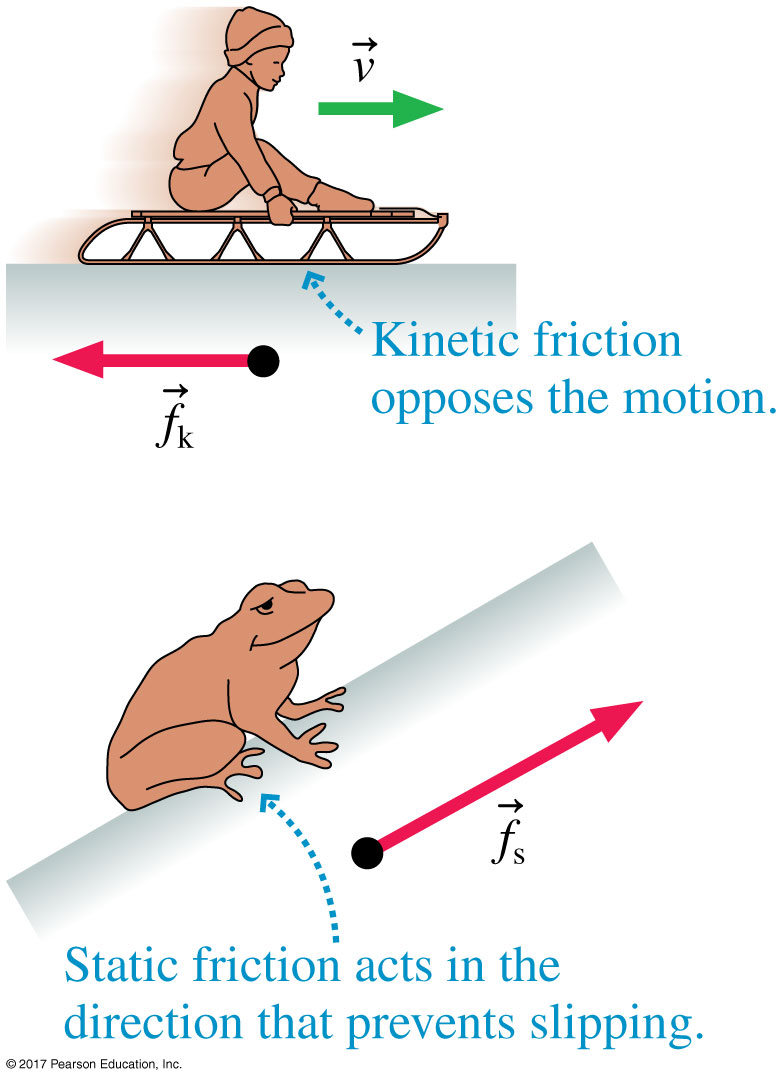
\includegraphics[width=\textwidth,trim={0 9cm 0 0},clip]{../figures/05_08_Figure.jpg}
\end{center}
\end{column}
\end{columns}
\end{frame}

\begin{frame}{Quick Check}
\begin{center}
   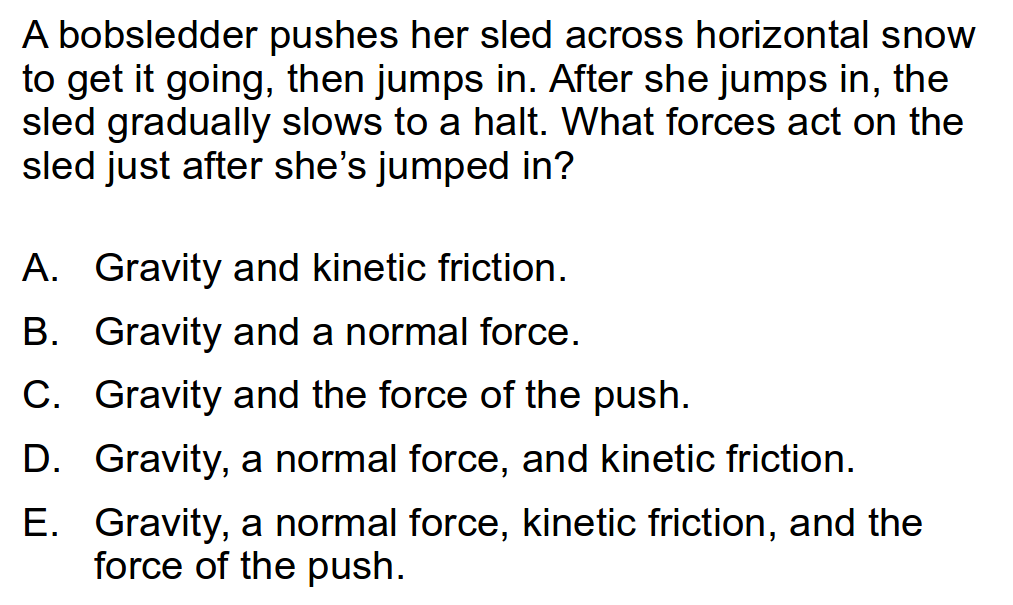
\includegraphics[width=\textwidth]{../figures/QC5_5.png}
\end{center}
\only<2>{\checkL{0.9cm}{6.1cm}}
\end{frame}

 \begin{frame}{Types of Forces - Static Friction}
\begin{columns}
\begin{column}{0.6\textwidth}
\begin{itemize}
   \item {\bf Static friction} is the contact force that keeps an object ``stuck" on a surface, and prevents relative motion. 
   \item The static friction force is directed {\it tangent} to the surface.
   \item Static friction points {\it opposite the direction} in which the object would move if there were no static friction.
\end{itemize}
\end{column}
\begin{column}{0.4\textwidth}
\begin{center}
   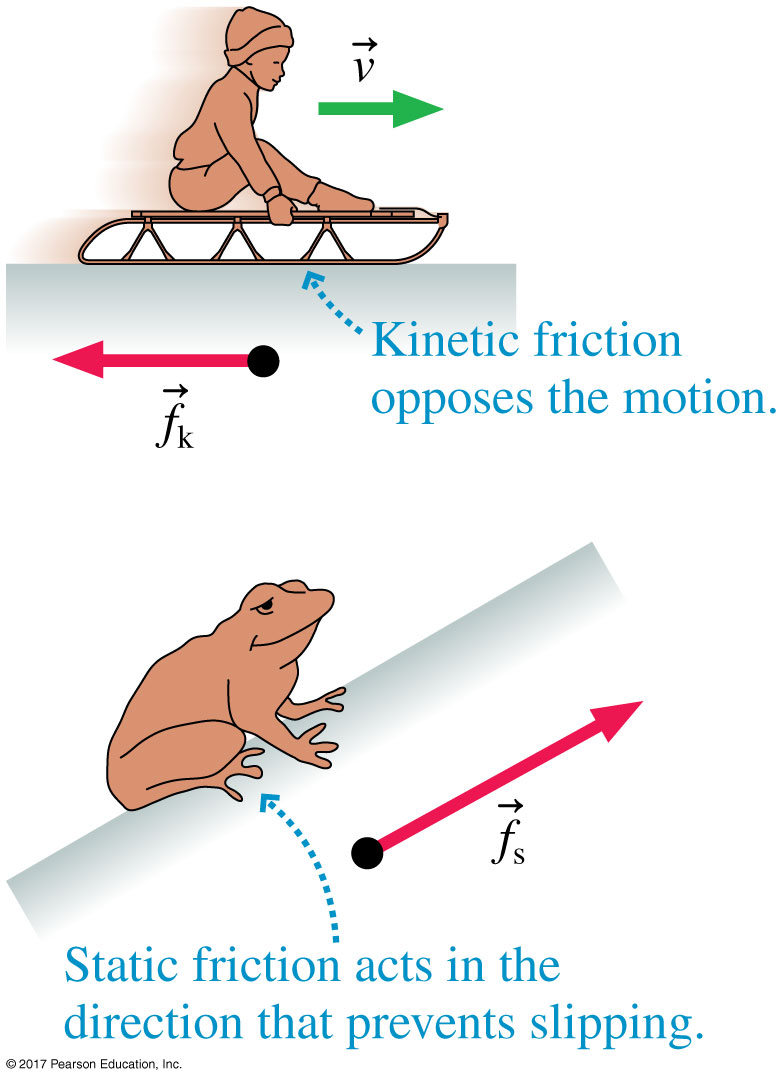
\includegraphics[width=\textwidth,trim={0 0 0 9cm},clip]{../figures/05_08_Figure.jpg}
\end{center}
\end{column}
\end{columns}
\end{frame}

 \begin{frame}{Types of Forces - Drag}
\begin{columns}
\begin{column}{0.4\textwidth}
\begin{center}
   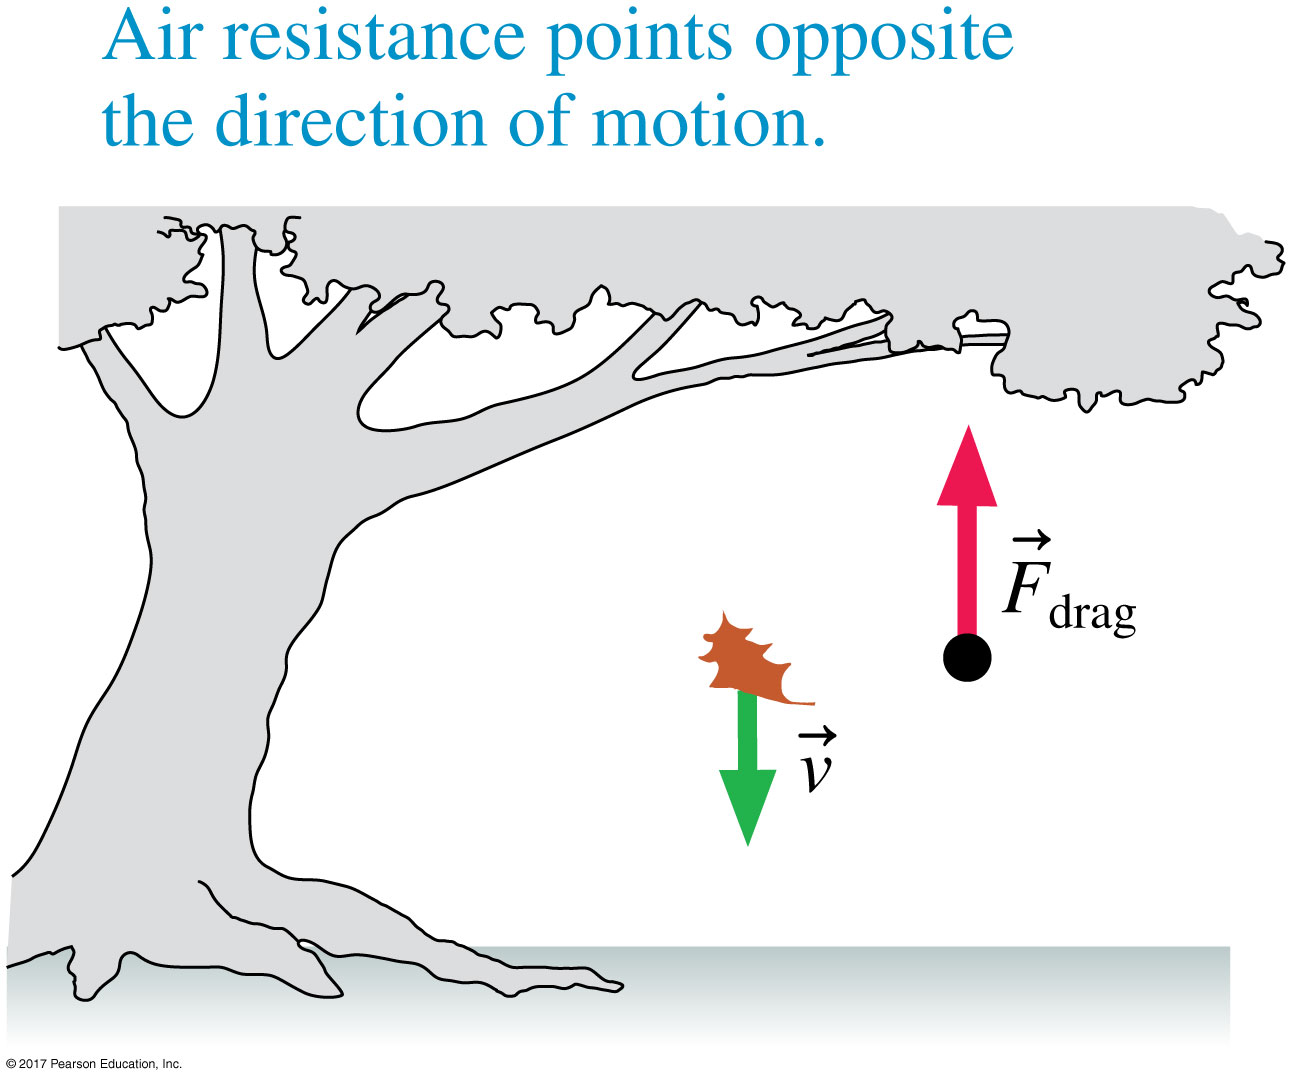
\includegraphics[width=\textwidth]{../figures/05_09_Figure.jpg}
\end{center}
\end{column}
\begin{column}{0.6\textwidth}
\begin{itemize}
   \item Kinetic friction is a resistive force, which opposes or resists motion.
   \item Resistive forces are also experienced by objects moving through fluids.
   \item The resistive force of a fluid is called {\bf drag}.
   \item Drag points opposite the direction of motion.
   \item For heavy and compact objects in air, drag force is fairly small.
   \item {\bf You can neglect air resistance in all problems unless a problem explicitly asks you to include it.}
\end{itemize}
\end{column}
\end{columns}
\end{frame}

\begin{frame}{Types of Forces - Thrust}
\begin{columns}
\begin{column}{0.6\textwidth}
\begin{itemize}
   \item A jet airplane or a rocket has a {\bf thrust force} pushing it forward during takeoff.
   \item Thrust occurs when an engine expels gas molecules at high speed.
   \item This exhaust gas exerts a contact force on the engine (We'll talk more about this in the future).
   \item The direction of thrust is opposite the direction in which the exhaust gas is expelled.
\end{itemize}
\end{column}
\begin{column}{0.4\textwidth}
\begin{center}
   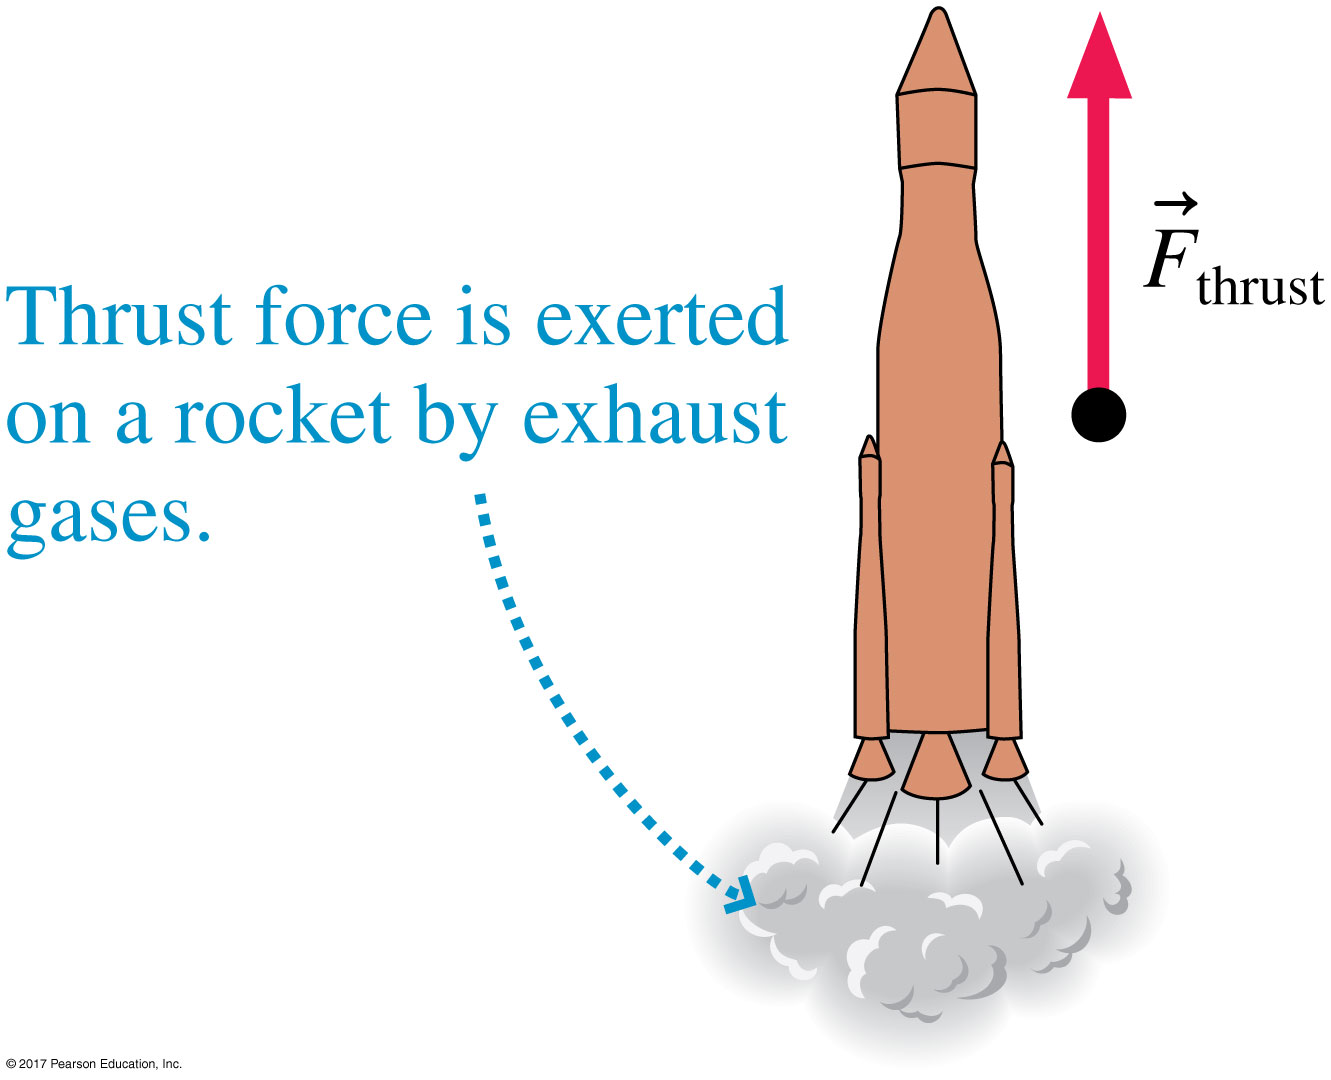
\includegraphics[width=\textwidth]{../figures/05_10_Figure.jpg}
\end{center}
\end{column}
\end{columns}
\end{frame}

\begin{frame}{Types of Forces - Electric and Magnetic}
\begin{columns}
\begin{column}{0.4\textwidth}
\begin{center}
   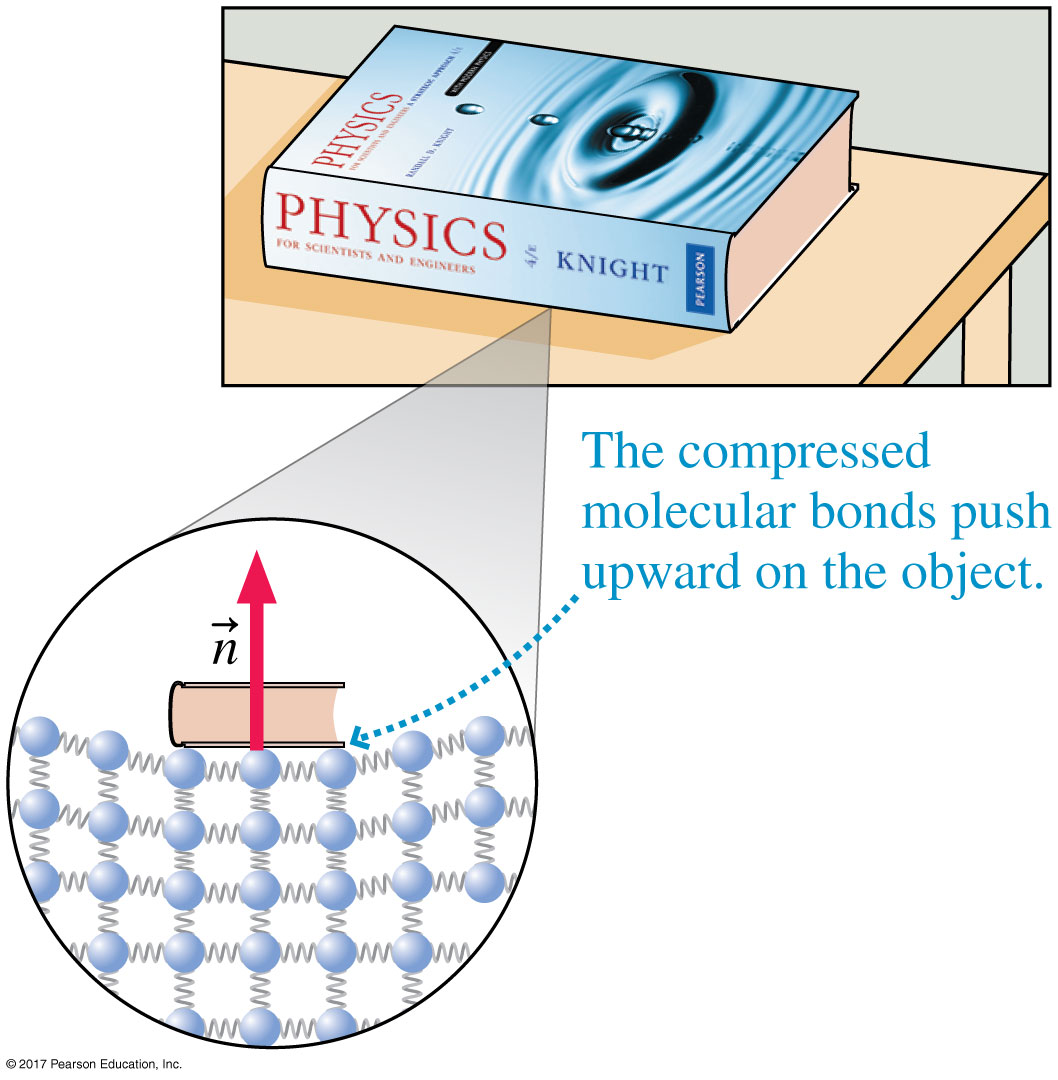
\includegraphics[width=\textwidth]{../figures/05_06_Figure.jpg}
\end{center}
\end{column}
\begin{column}{0.6\textwidth}
\begin{itemize}
   \item Electric and Magnetic forces exert long-range forces (like gravity).
   \item We aren't going to study these forces in the class, but you will in physics II.
   \item Bonds between particles in materials are due to these forces and thus the normal force, friction are really a types of electric and magnetic forces.
\end{itemize}
\end{column}
\end{columns}
\end{frame}

\begin{frame}{Types of Forces}
\begin{center}
   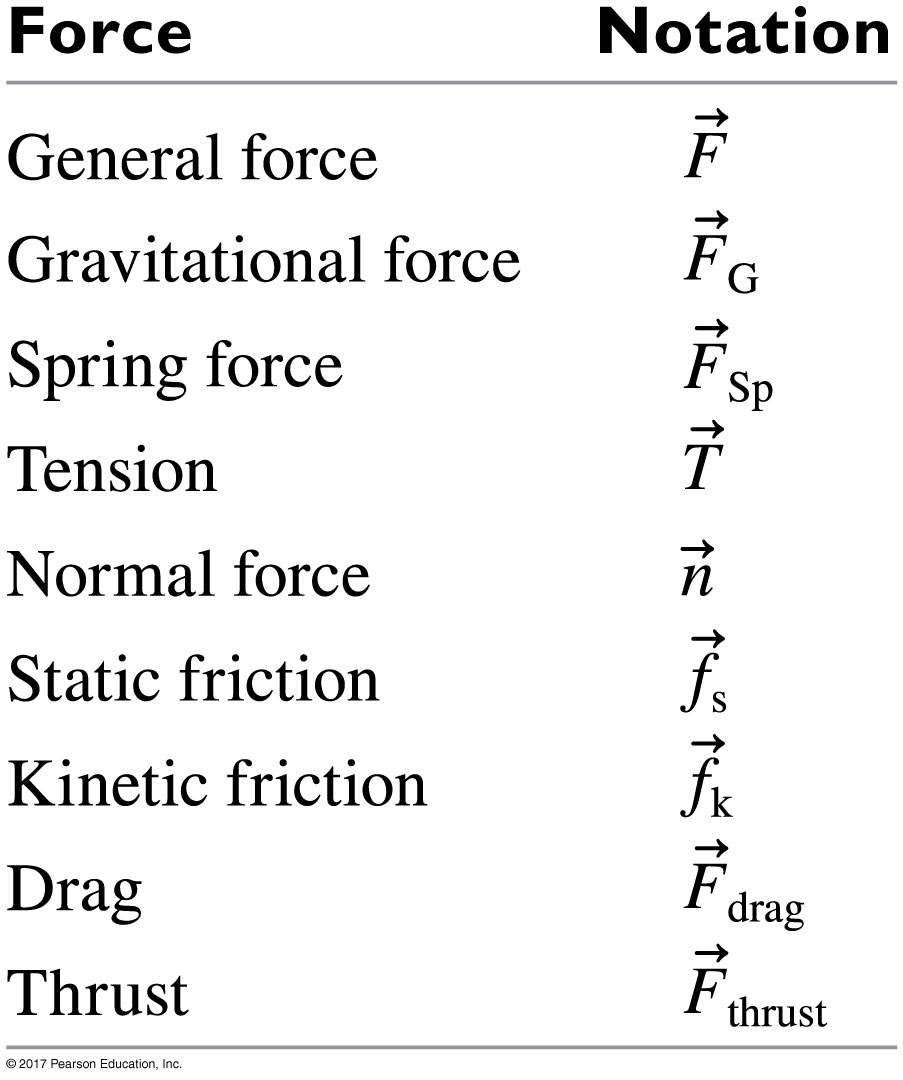
\includegraphics[height=0.9\textheight]{../figures/05_Pg116_UnTable.jpg}
\end{center}
\end{frame}

\begin{frame}{Identifying Forces}
\begin{center}
   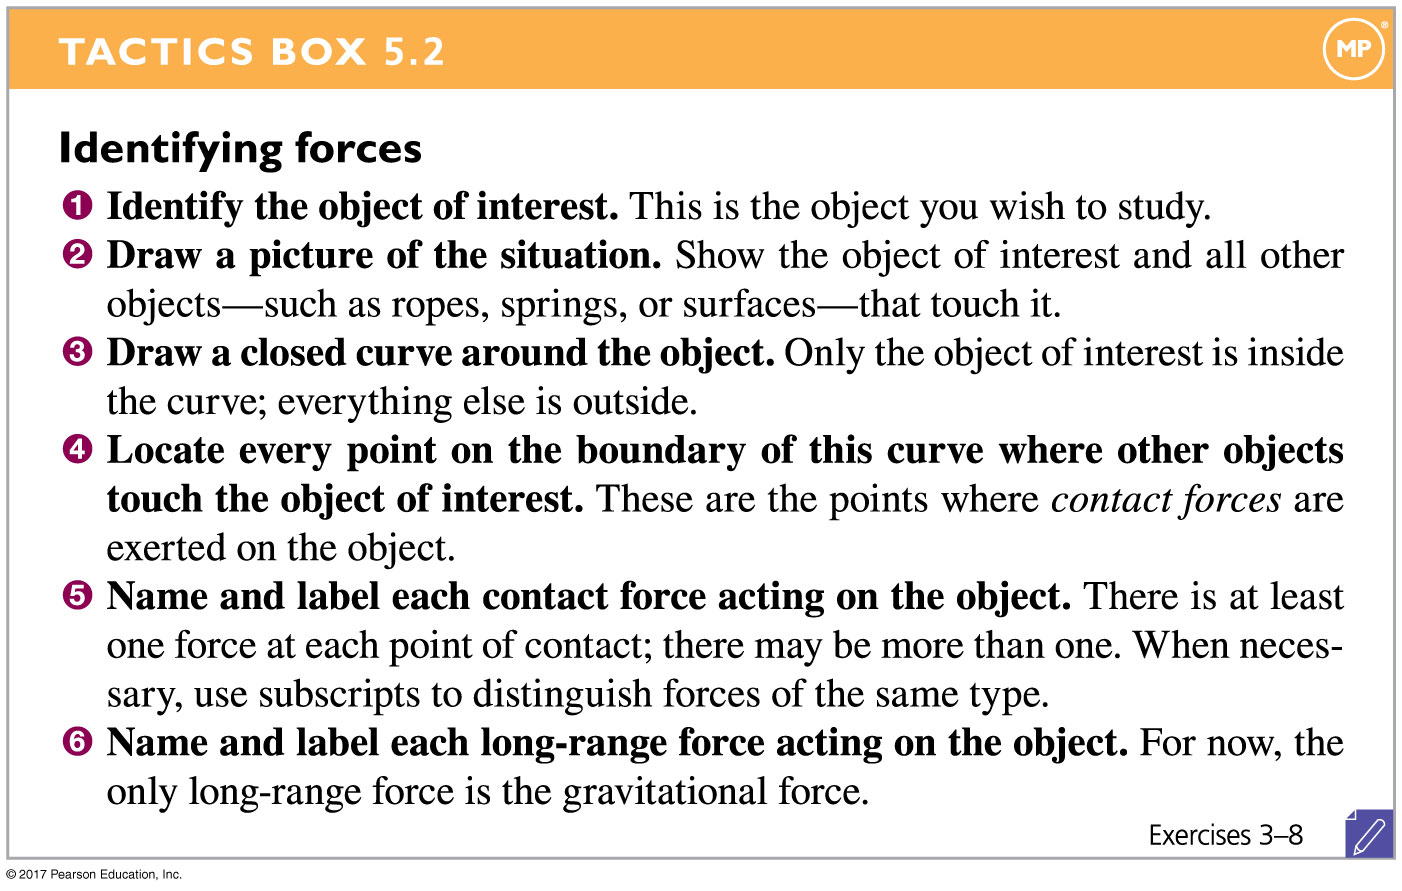
\includegraphics[width=\textwidth]{../figures/05_TacticsBox_02.jpg}
\end{center}
\end{frame}

\begin{frame}{Identifying Forces}
\begin{center}
   \only<1>{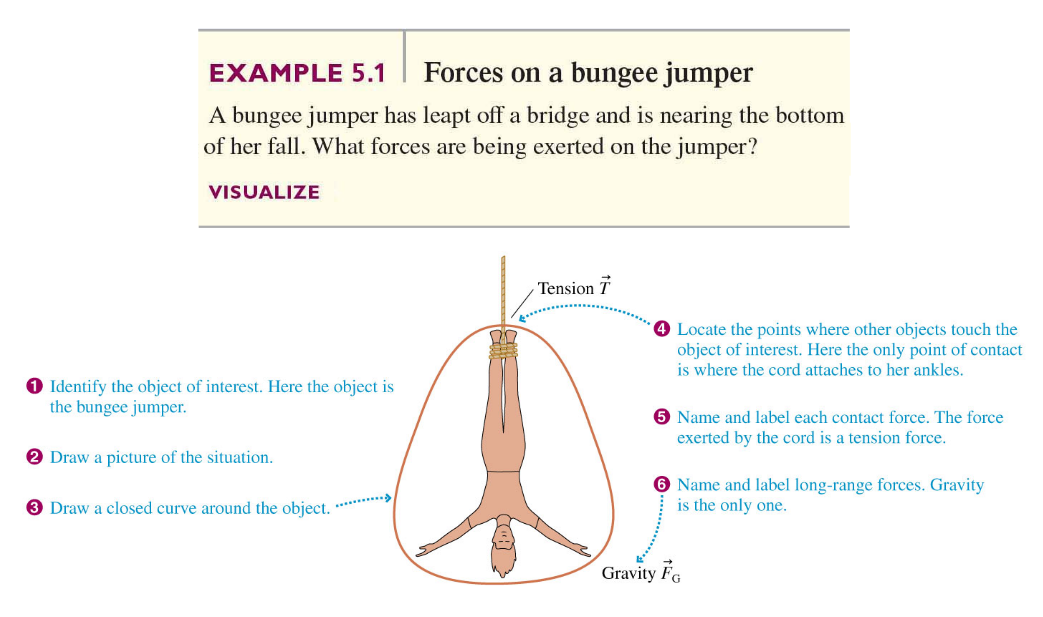
\includegraphics[width=\textwidth,trim={0 13cm 0 0},clip]{../figures/EX5_1.png}}
   \only<2>{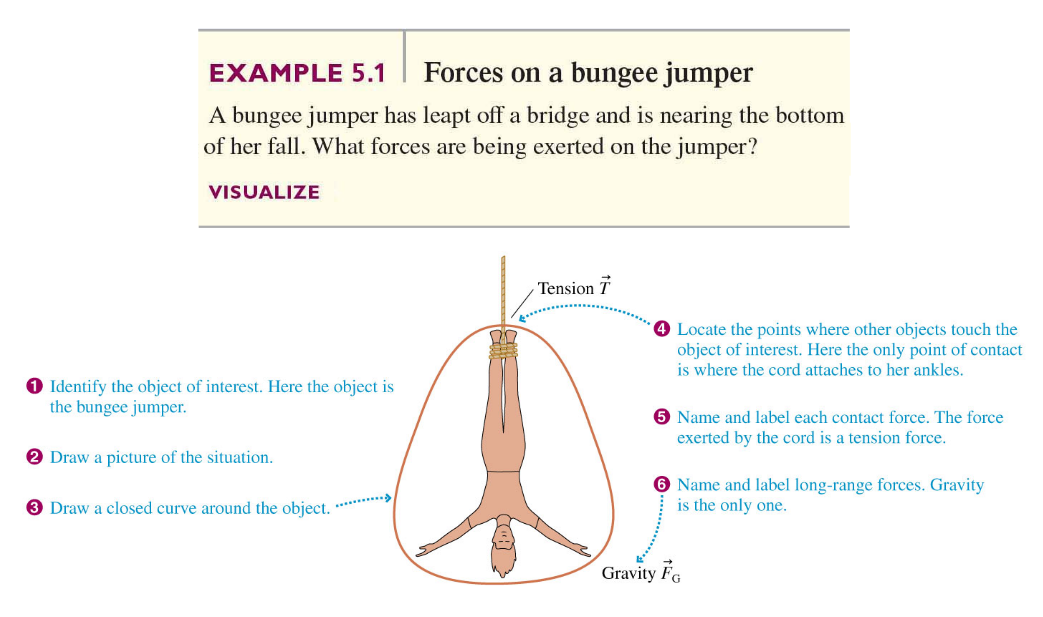
\includegraphics[width=\textwidth]{../figures/EX5_1.png}}
\end{center}
\end{frame}

\begin{frame}{Identifying Forces}
\begin{center}
   \only<1>{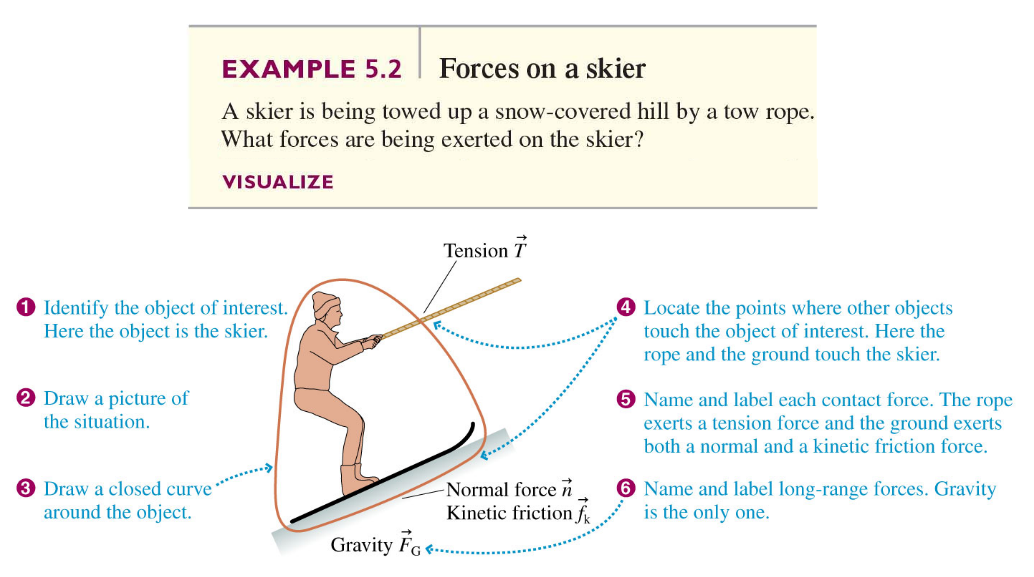
\includegraphics[width=\textwidth,trim={0 13cm 0 0},clip]{../figures/EX5_2.png}}
   \only<2>{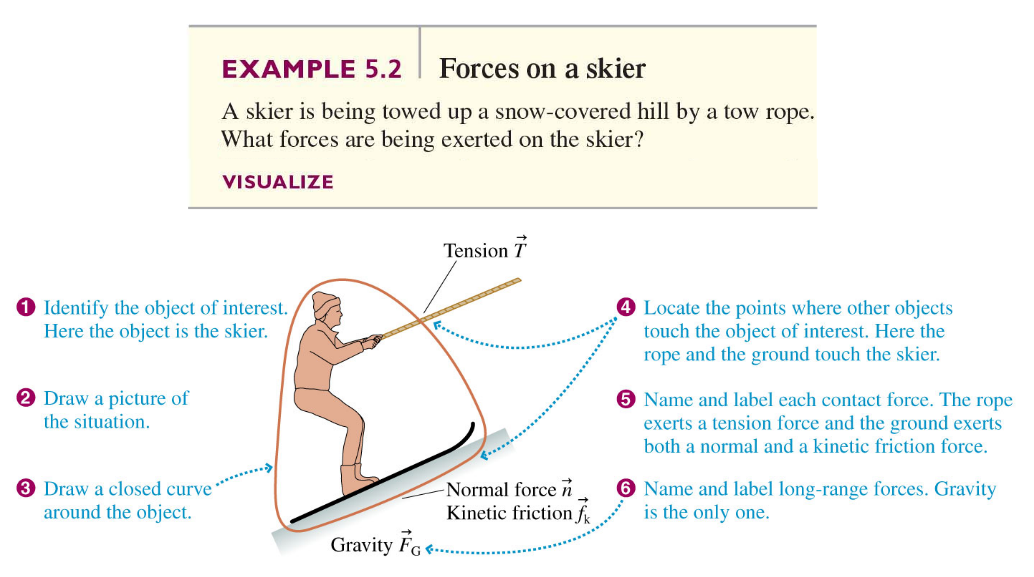
\includegraphics[width=\textwidth]{../figures/EX5_2.png}}
\end{center}
\end{frame}

\begin{frame}{Identifying Forces}
\begin{center}
   \only<1>{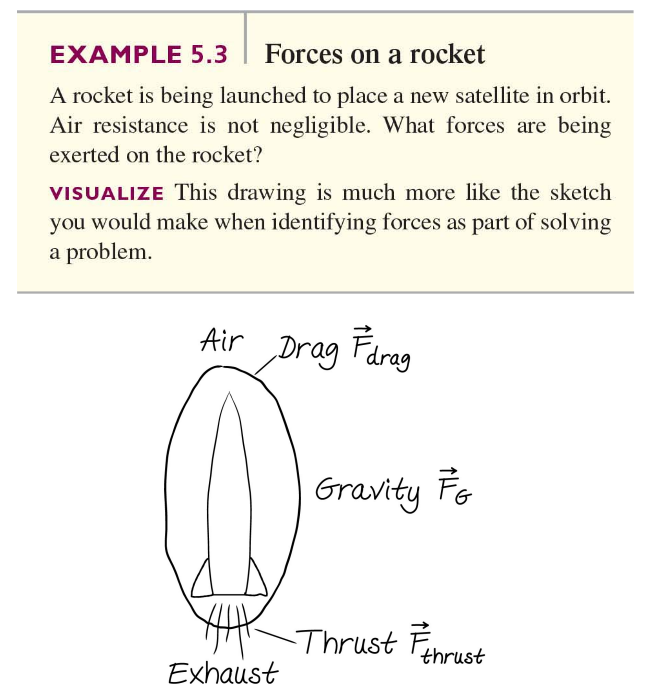
\includegraphics[width=0.7\textwidth,trim={0 13cm 0 0},clip]{../figures/EX5_3.png}}
   \only<2>{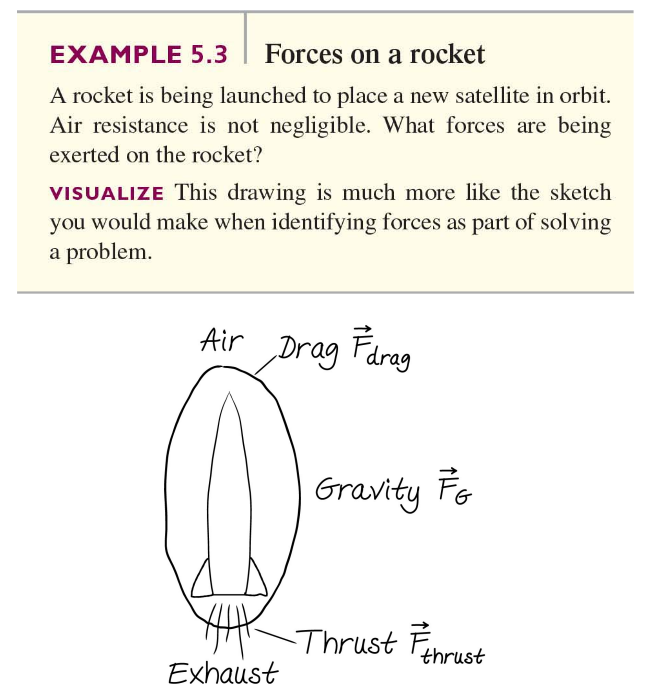
\includegraphics[width=0.7\textwidth]{../figures/EX5_3.png}}
\end{center}
\end{frame}

\begin{frame}{Picture References}
\tiny
None yet
\end{frame}

\end{document}
